% THIS IS SIGPROC-SP.TEX - VERSION 3.1
% WORKS WITH V3.2SP OF ACM_PROC_ARTICLE-SP.CLS
% APRIL 2009
%
% It is an example file showing how to use the 'acm_proc_article-sp.cls' V3.2SP
% LaTeX2e document class file for Conference Proceedings submissions.
% ----------------------------------------------------------------------------------------------------------------
% This .tex file (and associated .cls V3.2SP) *DOES NOT* produce:
%       1) The Permission Statement
%       2) The Conference (location) Info information
%       3) The Copyright Line with ACM data
%       4) Page numbering
% ---------------------------------------------------------------------------------------------------------------
% It is an example which *does* use the .bib file (from which the .bbl file
% is produced).
% REMEMBER HOWEVER: After having produced the .bbl file,
% and prior to final submission,
% you need to 'insert'  your .bbl file into your source .tex file so as to provide
% ONE 'self-contained' source file.
%
% Questions regarding SIGS should be sent to
% Adrienne Griscti ---> griscti@acm.org
%
% Questions/suggestions regarding the guidelines, .tex and .cls files, etc. to
% Gerald Murray ---> murray@hq.acm.org
%
% For tracking purposes - this is V3.1SP - APRIL 2009

\documentclass{style}

\usepackage{paralist}
\usepackage{graphicx}


\begin{document}

\title{Cache Oblivious B-trees}
%
% You need the command \numberofauthors to handle the 'placement
% and alignment' of the authors beneath the title.
%
% For aesthetic reasons, we recommend 'three authors at a time'
% i.e. three 'name/affiliation blocks' be placed beneath the title.
%
% NOTE: You are NOT restricted in how many 'rows' of
% "name/affiliations" may appear. We just ask that you restrict
% the number of 'columns' to three.
%
% Because of the available 'opening page real-estate'
% we ask you to refrain from putting more than six authors
% (two rows with three columns) beneath the article title.
% More than six makes the first-page appear very cluttered indeed.
%
% Use the \alignauthor commands to handle the names
% and affiliations for an 'aesthetic maximum' of six authors.
% Add names, affiliations, addresses for
% the seventh etc. author(s) as the argument for the
% \additionalauthors command.
% These 'additional authors' will be output/set for you
% without further effort on your part as the last section in
% the body of your article BEFORE References or any Appendices.

\numberofauthors{3} %  in this sample file, there are a *total*
% of EIGHT authors. SIX appear on the 'first-page' (for formatting
% reasons) and the remaining two appear in the \additionalauthors section.
%
\author{
% You can go ahead and credit any number of authors here,
% e.g. one 'row of three' or two rows (consisting of one row of three
% and a second row of one, two or three).
%
% The command \alignauthor (no curly braces needed) should
% precede each author name, affiliation/snail-mail address and
% e-mail address. Additionally, tag each line of
% affiliation/address with \affaddr, and tag the
% e-mail address with \email.
%
% 1st. author
\alignauthor
Salman Ahmad\\
\affaddr{MIT CSAIL}
\email{saahmad@mit.edu}
% 2nd. author
\alignauthor
Leilani Battle\\
\affaddr{MIT CSAIL}
\email{leibatt@mit.edu}
% 3rd. author
\alignauthor
Stephen Tu\\
\affaddr{MIT CSAIL}
\email{stephent@mit.edu}
}
% There's nothing stopping you putting the seventh, eighth, etc.
% author on the opening page (as the 'third row') but we ask,
% for aesthetic reasons that you place these 'additional authors'
% in the \additional authors block, viz.
\date{7 December 2011}
% Just remember to make sure that the TOTAL number of authors
% is the number that will appear on the first page PLUS the
% number that will appear in the \additionalauthors section.

\newcommand{\lhyperceil}{\lceil\lceil}
\newcommand{\rhyperceil}{\rceil\rceil}
\newcommand{\lhyperfloor}{\lfloor\lfloor}
\newcommand{\rhyperfloor}{\rfloor\rfloor}
\newcommand{\llangle}{\langle\langle}
\newcommand{\rrangle}{\rangle\rangle}

\newcommand{\Search}{\textsc{Search(k)}}
\newcommand{\Insert}{\textsc{Insert(k, v)}}
\newcommand{\Insertkonly}{\textsc{Insert(k)}}
\newcommand{\Scan}{\textsc{Scan(a, b)}}
\newcommand{\Delete}{\textsc{Delete(k)}}
\newcommand{\Succ}{\textsc{Succ(k)}}
\newcommand{\Pred}{\textsc{Pred(k)}}
\newcommand{\Member}{\textsc{Member(k)}}
\newcommand{\Range}{\textsc{Range-Query(k$_{i}$,k$_{j}$)}}

\maketitle
\begin{abstract}

This paper present a survey on cache-oblivious B-trees (CO B-trees). The CO
B-tree was first introduce by Bender et al in 2000. It is an external memory
data structure - meaning that it optimizes the number of memory transfers it
performs rather than the number of CPU instructions that it executions. Unlike
other external memory data structures, like the widely use B-tree, the CO
B-tree does not require any information about the number of level in the
machine's memory hierarchy, the block size and capacity at each level, or the
relative speeds at each level. Hence, the CO B-tree is ``cache-oblivious''.
Despite this, the CO B-tree is able to achieve the same optimal search bound
as the B-tree and near optimal insertion and deletion bounds as well. In this
paper we first describe the original CO B-tree and explain how it is able to
achieve its memory performance. We then present and analyze three followup CO
B-tree data structures that improved upon shortcoming of the original: the
cache-oblivious string B-tree, which introduces support for variable length
keys, the cache-oblivious streaming B-tree, which incorporates improvements to
the insertion bound at the expense of the search bound, and lastly, the
cache-oblivious concurrent B-tree, which introduces support for concurrency.

\end{abstract}

\section{Introduction}

\subsection{External Memory Algorithms}


Most algorithms assume an idealized model of computation that consists of a
single CPU, which performs instructions, and memory, which is a flat array
that can be read and written. However, in reality memory is not a flat array
but rather a hierarchy from super fast on chip caches, to slower main memory,
to even slower disks. When a program requests data, the data is found in the
memory hierarchy and typically carried up the hierarchy to the fastest memory
layer possible, usually a cache. The CPU is then able to access it to perform
any necessary operations. Unfortunately, this cache often has a small capacity
and once it is filled any new data requests cause some existing cached data to
be evicted. Transfering data from lower to higher levels in the memory
hierarchy often takes a long time. In fact, access times between the different
layers of the hierarchy can differ by many orders of magnitude and thus the
time to transfer data often dominates the overall runtime performance of an
algorithm. External memory algorithms are wary of this fact and aim to
optimizing the number of memory transfers it performs rather than the number
of instructions it executes. They often try to exploit the fact the memory
hierarchies transfer data in blocks rather than individual atomic units. Thus,
external memory algorithms are designed to not only limit the number of memory
transfers it performs but also preserve the locality of related data so that
when a memory access is performed, its cost is amortized.

\subsection{B-trees}

Since external memory algorithms are primarily concerned with accessing data,
it is no surprise that many external memory problems can be reduced to finding
a suitable data structure that efficiently implement certain operations. A
well known external memory data structure is the B-tree. At a high level, the
B-tree works by making each one of its nodes the same size as a memory block
in a particular level of the hierarchy. Furthermore, the fanout in the tree
(the number of children of a node) is proportional to the block size as well.
The B-tree incurs $O(log(N))$ memory transfers for \Search{}, \Insert{}, and
\Delete{} and is widely used in databases and filesystems.

\subsection{DAM vs CO}

The B-tree has two theoretical shortcomings. First, the B-tree is analyzed in
a two-level memory model called the Disk Access Machine (DAM) \cite{Aggarwal}.
However, in reality, computing architectures typically have memory hierarchies
that are much larger than two. The argument for the DAM model is that in
practice only one level in the memory hierarchy tends to dominate the
performance and thus a two-level memory model is sufficient for all intents
and purposes. However, this does mean that, theoretically, B-trees can begin
to incur an increasing number of memory transfers if the dominating level in
the hierarchy changes.

Additionally, the B-tree expects to know the block size of its memory layer in
advanced. B-Trees are implemented with parameterized code that needs to be
changed for every level in the memory hierarchy. Needless to say, this tuning
can be very difficult and error prone. Additionally, tuning this parameter may
even be impossible in certain heterogeneous computing environments.

The shortcomings of the DAM model gave rise to the cache-oblivious (CO) model
of computation. In the CO model an algorithm has no information about the
memory hierarchy. It does not know anything about the speed or the block size
of any level. Conceptually, the CO model allow algorithm designers to reason
about the simple two-level model like DAM but prove results for any arbitrary
multi-level memory hierarchy. This is because algorithms that perform well in
a CO model should, in theory, perform well regardless of changes in block
size, cache capacity, and cache speed. Consequently, CO algorithm should
gracefully scale to multi-level hierarchies as well.

\subsection{CO B-trees}

In \cite{BenderDemainColton} Bender et al. introduce the cache-oblivious
B-tree (CO B-tree). The CO B-tree is similar to the normal B-tree except that
it does not require explicit parameters about the memory hierarch.

The CO B-tree is able to achieve the optimal search bound of $\Theta(log(N))$
memory transfers, the optimal scan bound of $\Theta(N/B)$ memory transfers and
near optimal insertion and deletion bound of $\Theta(log_B N +
\frac{log^2{N}}{B})$. The CO B-tree was a seminal data structure that gave
rise to many others.

This paper provides a survey of the different types of CO B-trees and
discusses the various trade offs that they make. We start by analyzing the
original CO B-tree and explain how it works. This includes a detailed
description of the packed memory array (PMA) and strongly weight-balance
binary search trees (SWSBT) that are integral to the CO B-tree's memory
performance. Following this discussion we provide an analysis of the CO String
B-tree,a CO B-tree with variable length keys, the CO Streaming B-tree, a CO
B-tree that improves the cost of insertion at the expense of search, and the
CO Concurrent B-tree, which allows multiple processes to access the data at
the same time.

\section{Background}

\subsection{Original CO B-trees}
\label{sec:original}

Bender et al. first introduced a cache oblivious B-tree (CO B-tree) in
\cite{cobtree}. The CO B-tree achieves its number of memory transfers by structuring its elements as a
strongly weight-balanced search tree (SWBST). The SWBST is then laid out into
a packed memory array (PMA) using a van Emde Boas (vEB) layout. The SWBST and
PMA play crucial roles in the other cache-oblivious data structures that were
developed after the CO B-tree and thus are described at length in the next two
sections.

\subsection{Structure - SWBST}
\label{sec:structure}

\begin{figure}

\begin{center}
	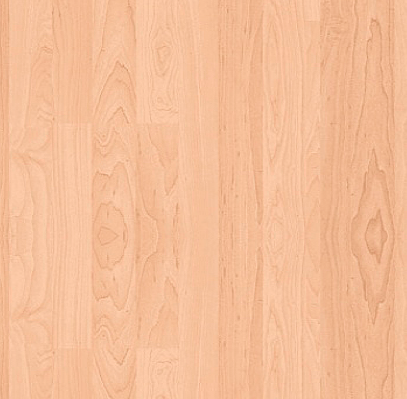
\includegraphics[width=0.8\columnwidth]{figures/veb.png}
\end{center}

\caption{An illustration of the van Emde Boas (vEB) layout}
\label{fig:veb}
\end{figure}


The ultimate goal of a CO B-tree is to reduce the number of memory transfers
while supporting \Search{}, \Insert{}, and \Delete{} operations. Thus, at a
fundamental level the CO B-tree still needs to maintain its data in some
structure. That structure is a balanced search tree. The search tree is laid
out according to a van Emde Boas (vEB) layout [???, ???]. The idea of a vEB
layout is fairly straight forward. Let $h$ denote the height of a tree. the
vEB layout splits the tree approximately at height $h/2$. This splits the
original tree into a ``top'' subtree and many ``bottom'' subtrees. Let $A$
denote the top subtree and $B_1... B_k$ denote the bottom subtrees. The vEB
layout is defined recursively using the order: $A, B1, ... B_k$. This layout
is also shown in Figure~\ref{fig:veb}.

A nice consequence of using a vEB layout is that it is known that it will use
$O(log_B N)$ memory transfers for searches [???, ???]. Thus, the CO B-tree has already
achieved the desired number of memory transfers for search queries. It
still remains to be shown that the CO B-tree achieves the desired number of
memory transfers for dynamic inserts and deletes.

It is known that the CO B-tree is going to use a balance search tree, but what
kind? This is where the strongly weight-balanced search tree becomes useful. The
weight of a node is $u$ is equal to the total number of $u$'s descendants plus
1. It can also be thought of as the sum of the weights of $u$'s children plus
1. Formally, $u$'s weight is: $w(u) = 1 + \sum_{v \in children} w(v)$.

Most weight-balanced search trees which requires that the heights of a node's
left and right subtrees are simply off by a constant factor. The SWBST enforces the
stronger property that a node at height $h$ in the tree (height is the node's
distance from the leaves; leaves have a height of 1) has $\Theta c^h$
descendants where $c$ is some constant. This property becomes important later
on when laying the tree out in memory (see Section~\ref{sec:layout}).

A known data structure that achieves this property is the ``weight-balanced
B-tree'' \cite{????}. The CO B-tree leverages this data structure to maintain
its elements. Before SWBST can be used, however, it remains to be proven that
it maintains the the $c^h$ descendants property even after inserts and
deletes.

The definition of a SWBST given in [????] provides us with this bound for the
weight of a node:

\begin{equation}
\frac{c^{h-1}}{2} \leq w(u) \leq 2c^{h-1}
\end{equation}

Lets now consider insertions. To insert an element into a WSBST we search down
the tree and find the natural place to insert the element - just like in any
tree structure. After inserting the element into some node $w$, we have to
check to see if any of $w$'s ancestors have become unbalanced by having a
weight greater than $2^{d-1}$. If such an ancestor exists, it follows that
every node along the path between that ancestor and $w$ will be un balanced as
well. Thus, we start with $w$ and move up the tree.

When we split a node, we naturally need to determine which children belong to
which of the two nodes. We cannot just divide the children evenly because it
may cause another violation. Thus, instead, we find the longest sequence of
elements such that the weight of that subsequence is $\lceil w(u)/2 \rceil$.
By doing this, we maintain the bound that $\frac{c^{h-1}}{2} \leq w(u) \leq
2c^{h-1}$. We cascade these changes up the tree until all of the ancestors
are balanced.

Deletions are supported in the exact same way, except, we check if a node has
a weight $w(u) < \frac{c^{h-1}}{2}$. In this case, we will merge two neighbors
together and proceed up the tree. There is one edge case that needs to be
handled. After merging, you may produce a new node that has a weight larger
than the bounds. If this happens we immediately split the node again. Thus,
this can be thought of as stealing nodes from a neighbor.

We have now shown that the SWBST achieves the desired property that the number
of descendants of a node is $c^h$. We can now show how to lay this tree out in
memory.

\subsection{Layout - PMA}
\label{sec:layout}


Now that we have our elements structured in a SWBST, we are still left with
mapping this tree to memory and proving that it achieves our desired number of
memory transfers. The packed memory array (PMA) was developed to solve this
problem [???]. There are three main costs that the PMA is concerned with.

Fist, the PMA needs to maintain open space in its memory for newly inserted
items. The PMA is able to accomplish this using $O(1 + (log^2 N) / B)$ memory
transfers. Doing so may seem like attempting to achieve contradictory goals:
maintaining the locality of elements while keeping space available for new
inserts. The PMA uses a technique described in [???]. At a high level, the PMA
maintains a windows into the array. When a window becomes too full or too
empty, the elements are spread out within the context of a larger window. Two
parameters are required, the window size and the threshold for trigger the
spreading out. However, these parameters are not related to the block size of
the memory level and thus do not violate the CO model of computation. Overall,
the PMA is able to keep extra space in $O(1 + (log^2 N) / B)$ memory
transfers.

Second, the PMA needs to handle the splitting and merging that will be caused
by the SWBST discussed in the previous section. The PMA is able to accomplish
this using $O(1 + (log N) /B)$ memory transfers. The proof is based on the
fact that each node has $c^h$ descendants (recall, this is the key property
that SWBST provided). Thus, merging or splitting a node will cause $c^h$ nodes
to move, requiring $O(1 + c^h/B)$ memory transfers. It follows from the
definition of SWBST in [???] that when a node is rebalanced, it will require
$c^h$ insertions or deletions until it is rebalanced again. Thus, the
amortized cost of each insertion and/or deletion is $O(1/B)$. When you split a
node, it may go all the way up the tree and thus overall it will incur $O((log
N) / B)$ memory transfers.

Third, the PMA needs to handle updating the parent and child pointers and may
become invalidated because of how the nodes moved around. The PMA is able to
update the parent and child pointers. If the pointers are all close together
in memory (e.g. within $B$ distance of each other) it is not big deal because
only a constant number of memory transfers are required. However, if they are
further apart the PMA introduces buffer nodes. The buffer nodes don't actually
do anything. All they do is serve to ``stretch'' the vEB layout so that nodes
do not move far away from one another. By using these buffers the PMA is able
to achieve a the pointer update cost using $O(1+ logB / \sqrt{B}) log^2 N)$
memory transfers.

Of these three terms, the dominating factor is maintaining room for newly
inserted elements - $O((log^2N)/B)$. We know that the SWBST achieves insertions and
deletions in $O(log_B N)$ if it is cache-aware. Thus, adding PMA makes
the SWBST cache-oblivious at the cost of incurring an additional $O((log^2N)/B)$ memory
transfers.

Therefore, overall, the CO B-Tree achieve insertions and deletions in $O(log_B N +
(log^2N)/B)$ memory transfers. However, it still achieves the optimal
$O(log_B N)$ memory transfers for searches, matching the performance of
ordinary, cache-aware, B-trees.

\section{Variable Length Strings}

\subsection{Motivation}
In order for B-trees to remain versatile, they must be able to accommodate various forms of data. However, traditional B-trees and string B-trees have suboptimal performance when variable length strings are used as keys. In addition, string B-trees do not support compression, and commonly used front compression is handled sub-optimally. Regular B-trees and string B-trees are not cache oblivious, and thus incur poorer performance as described previously in *cite original b-tree paper*. Range queries have poor performance in B-trees. In \cite{BenderFaKu06}, Bender et al. address these issues by designing a Cache Oblivious String B-tree (COSB-tree), which they argue works efficiently in these problem areas for variable length string keys. They also provide a modified front-compression scheme, which gives their approach the advantages of using less space and having improved locality within the compressed data.

Two experiments are performed, in which a regular B-tree implementation tuned to various block sizes is compared to a static COSB-tree implementation. The experiment involved measuring the amount of time required to perform: 440,000 and 450,000 inserts of random values, a range query of all values, and 1000 random searches. The results of the experiment show that COSB-trees outperformed B-trees most of the time for random searches, range queries and random inserts. However, some point between 440,000 and 450,000 inserts the COSB-tree had to rebalance the entire tree, causing it to fall behind in this measurement. However, Bender et al. argue that the experiment was biased towards the B-tree implementation, since the trees are "young", and thus still well organized. The COSB-tree implementation is also compared to Berkeley DB **cite berkeley db**, and achieves performance comparable to Berkeley DB with tuned parameters. The results seem to show that there is a window in which large and small-block size B-trees perform poorly, and that COSB-trees may be a reasonable alternative to improve performance.
\subsection{Description}

\subsubsection{General COSB-tree Structure}
The static COSB-tree consists of 2 layers: a centroid tree at the top, and an array of the keys stored in lexicographic order on the bottom. The leaves of the centroid tree contain pointers to keys in the array. The centroid tree is structured such that a search through the centroid tree identifies the local area of the desired key in the array. Then a sequential scan is performed across the array to find the key.

The Dynamic COSB-tree consists of 3 major components: a centroid tree at the top; a packed memory array (PMA) structure of hash data for the keys known as the \emph{hashdata} layer; and on the bottom a PMA structure for the original key values, compressed using an augmented version of forward compression known as the \emph{keydata} layer.

The centroid tree on a high level behaves similarly for static and dynamic COSB-trees. The leaves of the centroid tree point into the hashdata layer, where a sequential scan is performed to find the correct key by hash value. The hashdata layer points directly into the keydata layer, where the appropriate key is decoded, compared and returned.

In the following subsections, centroid trees are explained, and a summary of how to modify them to preserve weight balance in the dynamic case is provided. Two iterations on forward compression are also summarized to show how to incrementally add support for variable length strings as keys for dynamic COSB-trees. Lastly, the design and use of the hashdata and keydata are explained.

\subsubsection{The Dictionary Matching Problem and Centroid Trees} %todo:cite dictionary matching problem--sources in cosb-tree paper
In this approach to solving the dictionary matching problem, a dictionary $D$ of $N$ keys is preprocessed using hashing and divide-and-conquer via the construction of a centroid tree over the keys. This technique forms the basis for the Cache Oblivious String B-tree (COSB-tree) design. Consider the compacted trie $T$ of $D$. Bender et al. observe that there exists a centroid vertex $\rho$ in $T$ such that $\rho$ has between N/3 and 2N/3 descendants, inclusive. When searching for a key $k$ in the compacted trie, you traverse the tree as follows: for each node $y$ that you visit, if $y$ is a prefix of $x$, or $y$ matches $x$, continue on into the trie rooted at $y$ or \emph{down trie} of $y$. Otherwise traverse the trie resulting from excluding $y$ and its subtree. The \emph{centroid tree} is obtained by rooting the tree at \emph{centroid vertex} $\rho$, and making its children recursively defined \emph{centroid trees} of its up and down tries. 

At each step through the centroid tree, a consistent fraction of the nodes are eliminated from the search, resulting in an $O(logN)$ time bound when ignoring the time required to operate on keys. To make key comparisons faster, the keys are hashed and hash values are compared in place of the original key values. To avoid mismatches due to overlap in hash values, the original key values are compared after finding a match in hash values. The resulting time bound for \Search{} (interchangeable with \Member{}) is $O(||k||+logN)$. If each node in the centroid tree knows its successor and predecessor descendants, \Pred{} and \Succ{} can be achieved in $O(||k||+||k'||+logN)$, where $k'$ is the successor or predecessor of $k$. Note that the additive $logN$ incurred by the use of centroid trees can be avoided when using main memory. Centroid trees are used to capitalize on locality for the cache oblivious string B-tree design, described later in this section.

The centroid tree is built using $O(N/logN)$ keys, and the centroid tree is layed out in memory using a modified van Emde Boas (vEB) layout for weight-balanced binary trees. The \emph{hyperhyperfloors} of nodes are used as a guide for cutting the tree into equal-size subtrees for the vEB layout. The \emph{hyperhyperfloor} of x is denoted as $\lhyperfloor{}x\rhyperfloor{}$, and refers to rounding x down to the nearest power of a power of 2. This ensures trees of equal size on all \emph{levels of detail}, as the centroid tree is traversed.

The following approach is used to rebalance the centroid tree: Put all the elements in DFS or Euler tour order for the trie. Given this order, scan the trie to identify the centroid vertex, partition the trie into its respective up and down tries, and recurse on the up and down tries. The Euler tour order can be achieved via $O(\log{}N)$ scans, since the trie is only $O(\log{}N)$ deep. Thus updates have amortized cost of $O(1+\log^{2}N/B)$ memory transfers. Note that this doesn't include updating successor or predecessor pointers, which is described in more detail below.

The following approach is used for maintaining the vEB layout for centroid trees in the dynamic COSB-tree: first, weight balance is relaxed from a maximum weight difference of 2 between left and right subtrees, to a larger constant $c$. Thus a node $v$ only becomes out of balance every $\Omega(\textsc{weight(v)})$ insertions or deletions of descendants of v, reducing the frequency of rebuilds. The nodes are stored in a PMA structure, preserving order of the nodes using $\Theta(N)$space, apart from inserts and deletes. On insert or delete, the structure is scanned in both directions starting from the update point for sections of the array to rebalance based on a "density" threshold of the section. Rebalance here refers to evenly distributing the nodes across the section. To ensure that updating pointers isn't too expensive, any node included in the section must have its subtrees included. Specifically, the section is built up from the the lowest subtree level that contains or contained the update point, and neighboring subtrees are continuously added until either the density threshold is met or the entire current subtree layout at this "level of detail" is included. For example, suppose a node is inserted at the leaf of some lower recursive subtree $L_{i}$. To continue building up this section, $L_{i-1}$ or $L_{i+1}$ could be added. If all the lower recursive subtrees $L_{1}$,$L_{2}$,...,$L_{x}$ have been added, the top level tree $U$ is added. This corresponds to a subtree $L'_{j}$ one level above. Thus repeat this process until the density threshold is met, and then rebalance the tree. This approach depends on the fact that all the recursive subtrees at the same level of detail asymptotically have the same size, which Bender et al. prove about the hyperhyperfloor-based vEB layout described previously. This approach results in an amortized update cost of $O(1+(\log{}N)/B)$ memory transfers per update. In conjunction with the cost of rebuilds described above, this is only an additive $O(\log{}N/B)$ factor, so the overall bound is amortized $O(1+\log^{2}N/B)$ memory transfers.

Note that making the COSB-trees dynamic causes updates to successor and predecessor pointers in the centroid tree to be expensive. Thus the notion of ancestors is relaxed to the following (Lemma 10 in \cite{BenderFaKu06}): Let $\alpha$ be the parent node of $\gamma$ in the compressed trie. Then either $\alpha$ is a descendant of $\gamma$ or $\gamma$ is a descendant of $\alpha$. The proof is as follows: As you recursively traverse the trie, both $\alpha$ and $\gamma$ are in the up trie or down trie, until at some point one of them must be the centroid vertex. This is used to redefine what the predecessor/ancestor pointers refer to. The centroid may no loner point to the correct predecessor or successor with respect to the relevant subtrie, but one of the matched ancestors by construction must point to the correct predecessor/successor. Thus for the dynamic case, when dealing with successors and predecessors, $O(logN)$ ancestors' successor and predecessor pointers in addition to the successor and predecessor pointers of the node in question must be checked. However, this is an additive factor, so the same time bound for update described above is still achieved.

\subsubsection{Modifying Front Compression to Preserve Locality}
This section provides a brief summary of how front compression is modified to optimize compression and decoding for static and dynamic cache-oblivious string B-trees. Consider a sequence of $j$ keys to store $k_{1}$,  $k_{2}$, ...,  $k_{j}$. Without compression, this requires $\sum_{j}||k_{j}||$ space in memory. To compress these keys using front compression, let $\pi_{j}$ be the longest common prefix between $k_{j}$ and $k_{j+1}$. Now instead we store the keys as follows: 
\begin{center}
$k_{1}$,$||\pi_{2}||$,$\sigma_{2}$,$||\pi_{3}||$$\sigma_{3}$,...,$||\pi_{j}||$,$\sigma_{j}$
\end{center}
where $\sigma_{j}$ is the suffix of $k_{j}$ after removing the first $\pi_{j}$ bits. This saves almost $\sum_{j}||\pi_{j}||$ memory. However, since decoding $k_{j}$ involves concatenating the first $\pi_{j}$ bits of $k_{j-1}$ to $\sigma_{j}$, $k_{j-1}$ must be decoded. $k_{j-1}$ may depend on previous keys as well, making $k_{j}$ expensive to decode.

The goal of modifying front compression is to maintain some of the space benefits to compression while reducing the high decoding cost and keeping the size of D small. Bender et al.  provide a modification for static COSB-trees that reduces the high decoding cost of front compression of D to $O(1+||k||B)$, with size $O(\llangle{D}\rrangle{})$ after compression. The modification works as follows: Let $c = 2 + \epsilon/2$, and let $k_{1}$ be the first key added to the compression stream. For each subsequent key $k_{i}$, if $k_{i}$ can be decoded with just the last $c||k_{i}||$ characters, add $\pi_{i}$,$\sigma_{i}$ like before. Otherwise, add 0,$k_{i}$, which means add $k_{i}$ to the stream in its uncompressed form. By construction, this scheme guarantees that any key $k_{j}$ can be decoded in $O(1+||k||B)$ memory transfers.%todo: add something about why this isO(<<D>>)?

However, the above modification falls short for anticipating insertions and deletions. The previous modification relies on each key being decoded within $c||k^{*}||$ elements of the compressed array, but this is no longer guaranteed when new keys can be inserted to the left of $k$. To make the locality-preserving front compression technique suitable for dynamic COSB-trees, Bender et al. modify the algorithm to include an extra copied prefix for each key. Consider the $3c||k||$ characters that would be to the left of a new key$k^{*}$ after insertion. Let $k'$ be the key at the end of this range. The idea is to prevent the insertion of $k^{*}$ from affecting any non-copied keys just to the right of $k'$, since this could potentially increase their decode cost. Compute the length $l$ of the largest common prefix (lcp) between $k^{*}$ and $k'$, and compare $l$ to all the other lcp's in this range. $l$ represents the minimum length for any lcp between $k^{*}$ and $k'$, since the keys are stored in lexicographic order. If there is a copied prefix of length at least $l$ or a copied key within this range, insert $k^{*}$ as usual. Inserting $k^{*}$ will have no negative effect in this respect, since the decode length is effectively reset by the copied key or prefix like before. However, if inserting $k^{*}$ causes the minimum length of the lcp's in this range to increase, we need to fix the compression. To do this, we update the lcp of the key directly to the right of $k^{*}$ and store an extra copy of this lcp with $k^{*}$ itself. In this way, we can charge the work of copying extra prefixes for a new key to the appropriate number of elements before it. This number is determined by the length of the extra copied prefix stored with the key.

\subsection{Operators}
%todo: figure out how to do range queries from this paper somehow...
The operations supported are dictated by the Dictionary Matching problem. These operations are: \Search{} (synonymous with \Member{}), \Pred{}, \Succ{}, and \Range{}. The behavior of each operation for dynamic COSB-trees is described below. \Insertkonly{} and \Delete{} are also supported but not described here.

\Search{}: works as follows for a given key $k$. Compute the hash value for $k$ and call it $\rho$, and traverse the centroid tree of the COSB-tree using $\rho$ to obtain the successor $\rho_{s}$ and predecessor $\rho_{p}$ of $k$. Index into the hashdata layer and perform a sequential scan across the PMA structure from $\rho_{p}$  to $\rho_{s}$ to find $\rho$. On a match with value $\rho'$, index into the keydata layer and decode $\rho'$ to obtain the resulting key $k'$. If $k' = k$, return true. If $k' \ne k$ or $k$ was not found during the sequential scan return false.

\Pred{},\Succ{}: works in the same way as \Search{} until the sequential scan in the hashdata layer. When scanning the hashdata layer, look for $\rho_{p}$ or $\rho_{s}$, respectively, in place of $\rho$, and compare the appropriate keys in the keydata layer. 

\Range{}: The paper doesn't say, but presumably this is very similar to \Search{}. Let $k_{b}$ be the beginning of the range and let $k_{e}$ be the end of the range. Hash the range keys and identify the predecessor of $\rho_{b}$ and the successor of $\rho_{e}$ using the centroid tree. Scan the hashdata layer across from  $\rho_{b,p}$ to  $\rho_{e,s}$. Only start noting the beginning of range when the first key with hash value after $\rho_{b}$, and stop once we reach the first key with hash value after $\rho_{e}$. Decode and return the set of keys within the given range in the keydata layer.

\subsection{Complexity}
\Search{} takes $O(1+\log_{B}N+||k||/B)$ memory transfers with high probability (w.h.p.). Traversing the centroid tree requires  $O(1+\log_{B}N)$ memory transfers, since the tree is built using$O(N/logN)$ keys and is balanced. Once in the hashdata layer, we are already within $O(logN)$ keys of $k$. Thus the local scan requires $O(1+(||k||+\log{}N)/B)$ memory transfers. Obtaining $k$ from the keydata layer requires no more memory transfers than the scan in the hashdata layer. The \Pred{} and \Succ{} operations are almost identical in behavior to searches, and thus only have the added cost of having to operate on $k'$, where $k'$ is the predecessor or successor, respectively. These operations as a result take $O(1+\log_{B}N+||k||/B+||k'||/B)$ memory transfers w.h.p.. Similarly, range queries take $O(1+\log_{B}N+(||k||+||k'||+\llangle{}Q\rrangle{})/B)$ memory transfers, where in this case $k'$ is the other end of the range and $Q$ is the set of keys within the given range.

\Insertkonly{} and \Delete{} w.h.p. require $O(1+\log_{B}N+\log^{2}N||k||/B)$ memory transfers. As mentioned previously, due to rebuilds updates have amortized cost of $O(1+(\log^{2}N)/B)$ memory transfers. The rest of the cost for insertions and deletions is due to having to find the correct key to delete or location for insert, which can be seen from the cost of \Search{}.

\section{Streaming B-trees}

\subsection{Description}

While B-trees achieve an optimal bound for the number of memory transfer for
search, they do not perform as well for updates and insertions. The
buffered-repository tree (BRT) is a common alternative to the B-tree that
achieves an improved amortized $O(log(N)/B)$ memory transfers for inserts
compared to the $O(log_{B+1}N)$ memory access of B-trees. Of course, the
B-tree and BRT are analyzed with the DMA model and are not cache-oblivious.

This search vs insertion trade off also exists in the cache-oblivious model.
The original BO B-tree described in Section~\ref{sec:original} is designed to
optimize for the search in this trade off. However, Bender et al. propose two
data structures that and achieve the opposite end: the shuttle tree and the
cache-oblivious lookahead array (COLA) \cite{BenderFaFi07}. These two data
structures are refereed to as ``streaming B-trees'', indicating how they are
optimized for insertions at the cost of search.

\subsection{Shuttle Trees}

The shuttle tree is similar in layout and structure as the original CO B-Tree.
It uses a strongly weight-balanced search tree described previously (see
Section~\ref{sec:structure}) that is laid out in a vEB (see
Section~\ref{sec:veb}) layout into a PMA (see Section~\ref{sec:layout}). A
notable difference between the shuttle tree and the CO B-tree is that the CO
B-tree splits the tree at height $h/2$ when creating the vEB layout while the
shuttle tree splits at height $F_k$, where $F_k$ is the $kth$ Fibonacci number
that is stickily less than the height of the tree. Thus if a tree's height
happens to be a Fibonacci number, $F_k$, then the shuttle tree will choose to
split the tree at height $F_{k-1}$. The top and bottom ``halves'' produced by
this split are organized just like before and shown in Figure \ref{fig:veb}.

\begin{figure}

\begin{center}
	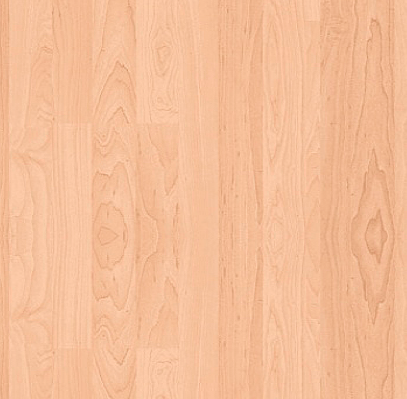
\includegraphics[width=0.8\columnwidth]{figures/veb.png}
\end{center}

\caption{An illustration of how the shuttle tree determines the size of a node's linked list}
\label{fig:buffers}
\end{figure}


At a high level, the shuttle tree improves the efficiency of insertion by
adding buffers to each node in the tree. In fact, shuttle tree nodes have a
linked list of buffers rather than just a single buffer like the BRT. Each of
these buffers is another shuttle tree. The a shuttle tree node enforces two
constraints: the length of its linked list as well as the overall height (and
thus capacity) of each of the buffered shuttle trees contained within its
linked list.

The length of a node's linked list is related to the node's height in the
tree. A node has a buffer for every time it the leaf of a sub trees that is
split when creating the vEB layout. This idea is illustrated in Figure
\ref{fig:buffers}.

The shuttle tree's node's buffers have a maximum capacity that is enforced by
bounding its height. The size of the buffers increases going across the linked
list. Thus, a node's first buffer is smaller than its last buffer. The maximum
height of a buffer is given by $F_{H(k)} = F_{k-2 \lceil log_{\phi} k \rceil}
$ where $\phi$ is the golden ratio and $k$ is chosen such that $F_k$ =
$\xi(h)$ and $\xi(x)$ is defined recursively. If $h$ is a Fibonacci number
then $\xi(h) = h$ and otherwise $\xi(h) = \xi(h-f)$ where f is the largest
Fibonacci number less than $h$. The maximum height of an individual buffer is
related to the size of the recursive subtree for which the node is a leaf.
Since the recursive subtrees are split based on the largest Fibonacci number
less than $h$ (as described previously) it follows that the buffer sizes are
also based on Fibonacci numbers.

\subsubsection{Operators}

The operations that are described by Bender et al. for the shuttle tree are
\Search{}, \Insert{}, and \Scan{}. An explicit discussion on \Delete{} is
missing; however, it is assumed that it is symmetric to \Insert{}.

\Search{} and \Scan{} work virtually the same way as the CO B-tree. The only
difference is that you have to search a child node's buffer before following
the pointer down the tree.

\Insert{} is also similar to the CO B-tree except you buffer elements as you
add them. When you insert an element you move down the tree from the root to
leaves and stop when you find a node that has a buffer (note that because of
the nature of Fibonacci numbers that it is possible that a node does not have
any buffers). You then attempt to insert the element into the smallest buffer
in the node's linked list. If this insertion causes the buffer to overflow
(e.g. the height of the buffer exceeds its maximum), you move all of the
elements from this buffer to the next largest buffer. When the largest buffer
overflows you take all of its elements and ``shuttle'' them down the tree.
Eventually you will hit a leaf node and inserting here may cause the balance
constraints on the SWBST to become invalidated. The shuttle tree rebalances
itself just like any other SWBST: the leaf node is split into two and this
split cascades up the tree until balance is restored.

The shuttle tree also needs to take care of the buffers belonging to a split
node. When a node $u$ is split into two nodes $u_1$ and $u_2$ the shuttle tree
immediately allocates enough space for all of the $u_2$'s buffers ($u_1$
simply reuses the space allocated for $u$'s buffers). We then scan over $u$'s
buffers and find the ones rooted in $u_1$ and $u_2$ and move them
respectively. This can be achieved by a single scan.

The core problem of maintaining room for inserts, bounding the costs of
merging and splitting, and bounding the costs of updating parent and child
pointers in the shuttle tree is achieved using the same PMA used with the CO
B-tree. This is decried in detail in Section~\ref{sec:layout}.

\subsubsection{Complexity}

\Search{} uses $O(log_B N)$ memory transfers where $N = \Theta(c^{F_k})$ and
$c$ is your fanout. Note that $c$ is not treated as a constant since this is a
cache-oblivious data structure. This bound is achieved by searching over the
top and bottom recursive subtrees at each level when traversing the tree. A
key trick is that when you visit a node you only search its largest buffer
(that last buffer in the linked list for that level). The smaller buffers will
be visited eventually as you recurse down the tree. Eventually you will get
down to a single subtree that can fit into $O(1)$ blocks and thus can be
searched with $O(1)$ memory accesses. Since the fanout is proportional to our
block size it will take us $O(log_B N)$ block accesses until we get down to a
subtree and thus, by induction, the worst case runtime is $O(log_B N)$.

% TODO - redo the insert section. Namely, include a discussion on how the
% shuttle tree maintains its structure dynamically. I mention the node
% splitting from pg 85 in the paper but do not include that in the analysis. I
% should basically mention that the cost of dynamically maintaining the
% shuttle tree O(logN / B) is not greater than the PMA log^2 N / B and thus
% the dynamic updates do not change the number of memory tranfers.

\Insert{} uses $O(log_{B+1} N / B^{\Theta(1/(loglogB)^2)} + (log^2 N) / B)$
memory transfers. This improvement over the CO B-tree is achieved because the
shuttle tree's buffers are used to maintain locality of the elements long
enough to amortize the cost of moving them down the tree and possibly into
another memory block. The proof is based on the fact that when an element is
moved from one block to another it is due to either a leaf node splitting or a
node's buffer overflowing. Recall that when inserting a new element causes a
buffer to overflow, all of the the elements from that buffer move down the
tree, not just the single one that caused the overflow. Thus, the cost of
inserting an element is amortize by the number of elements in a node's largest
buffer. The number of elements in the largest buffer is
$B^{\Theta(1/(loglogB)^2)}$ leading to the $B^{\Theta(1/(loglogB)^2)}$ factor
in the big-Oh notation.

\Scan{} uses an amortized $O(L/B)$ memory transfers to scan in $L$ consecutive
elements. This cost obviously does not include the single \Search{} operation
that is required to find the first starting element of the range. Once that
first element's block is transferred, the shuttle tree proceeds by traversing
the tree and scanning in elements. Since the vEB layout enforces the spatial
locality of nearby nodes in the tree, the shuttle tree only has to read in a
new block once every $B$ memory accesses. Thus, each individual memory access
is is amortized to $1/B$ and the overall number of memory transfers is
$O(L/B)$.

The last thing that is worth mentioning is that the overall space requirements
of the shuttle tree is $O(n)$. The high level intuition for this proof is that
the majority of the buffers are really small and thus do not impact the
overall size of the tree.

\subsection{COLA}

The cache-oblivious lookahead array (COLA) is actually quite different from
the other cache-oblivious data structures seen so far. Instead of an explicit
tree structure with child and parent pointers, the COLA is organized as a list
of arrays or levels. Each array has size $2^k$. Furthermore, each array is
either completely full or completely empty. As such, the COLA is very similar
to the binomial list structure described in \cite{BentleySaxe}.

\subsubsection{Operators}

The operations supported by COLA are \Search{}, \Insert{}, and \Scan{}. Once
again, \Delete{} can be inferred symmetrically from \Insert{}.

\Insert{} works by initially inserting an element into the first-level array.
This array has size $2^0 = 1$, thus the element is in an array on it own.
Whenever you insert an element you check to see if there is another array of
the same size (this can be though of as checking to see if there is another
array in the same level). If there is another array with the same size, the
COLA merges the two together in sorted order. This merging will produce a new
array that is twice the size and thus goes into the next level. The COLA
continues to merge until there are no two arrays of the same size.

\Search{} can naively be performed by simply scanning each of the levels in
the COLA. Since everything is sorted the COLA could can use a binary search to
quickly find the element it is looking for. However, this is not very
efficient. As an improvement COLA, as the name suggest, uses look ahead
pointers to reduce the number of memory accesses required. Every 8th element
from the $(k+1)$st level exists in the $k$ level array in its proper sorted
location. This element also contains a pointer to its real location in the
$(k+1)$st level. Thus this pointer is referred to as ``real lookahead
pointer''. Additionally, each every 4th cell in $k$th level array contains two
pointers pointing to the next and previous ``real lookahead pointers'' on this
level. The next and previous pointers are referred to as ``duplicate lookahead
pointers''. To search a level the COLA performs a binary search within an
appropriate range, determine the range in the next level using the ``duplicate
lookahead pointers'' and then recursively cascade up the tree.

\subsubsection{Complexity}

\Insert{} achieves an amortized $O(log N / B)$ memory transfers. The proof is
based on the far that an element will never be merged more than $O(log(N))$
times. This is because at that point it will be in the last array.
Additionally, the first $log(B)$ merges that a element participates in uses a
constant number of memory transfer since we can assume that the relevant
blocks are already cached. Thus, we only need to worry about memory transfers
when we merge levels that have size greater than $B$. If the size of the array
is $k$ then the cost of merging is $O(k/B)$ and thus the amortized cost of a
merging a single element is simply $1/B$. Since we just proved that an element
will only be merged $O(log(N))$ time, it follows that the overall amortized
memory transfers to insert an element is $O((log N)/B)$.

\Search{} achieves $O(log N)$ memory transfers. The proof uses induction to
show that the COLA never needs to search more than eight elements on each
level. Since there are $O(log(N))$ levels and since eight is a constant, it
follows that overall, search uses $O(log N)$ memory transfers. The fact that
only eight elements need to be search per level is shown through induction.
The base case is trivial. The first three levels of the COLA each have at most
eight elements (note that these elements are either actual real elements or
lookahead pointers). The COLA can obviously search these levels with no more
than eight member transfers. As the COLA follows lookahead pointers to the
higher levels, it will eventual get to a level where $k \geq 3$. Note that the
COLA does not ``enter'' this level at the start of the array; rather, its
arrived here by following the real lookahead pointers from the levels below
and thus is at some index $i$ that contains an element $e_i$ such that $e_i <
e$ and $e$ is the element being searched for. The goal at this point is to
find a new $i$ such that $e_i \leq e < e_{i+1}$. Once this $i$ is found the
duplicate lookahead pointers can be used to locate the ``next'' and
``previous'' real lookahead pointers in the next level. The two real lookahead
pointers are used to and restrict the search in the next level. Recall that at
each level in the COLA every eighth element in a level is present in the
previous level. Thus, it follows that in next level only 8 elements need to be
searched. Furthermore, since the current level was reach from a lower level,
it follows that only 8 elements need to be search on this level to find the
appropriate $i$. Thus, overall, the COLA uses $O(8log(N)) = O(log(N))$ memory
transfers.

\subsubsection{Performance}

In experimental results, the COLA achieved significant improvements over
normal (cache-aware) B-trees, performing 790 times faster. However this
improvement comes at the cost of sorted inserts and normal searches. Sorted
inserts are 3.1 times slower and searches are 3.5 times slower. Nevertheless,
these experimental results indicate that the the COLA is a suitable data
structure when random insertions are common.

\section{Concurrency}

\subsection{Motivation}
B-trees are often used as an indexing data structure for various
database and file systems. Thus, for a cache-oblivious B-tree data structure
to be of practical value, it must be able to handle concurrent access and modification
of its internal state. The straw-man solution is to simply ensure mutual exclusion
on the entire data structure; this approach, however, yields poor performance.

Various concurrency schemes for traditional cache-aware B-trees have been
proposed \cite{BayerS77, LehmanY81}. We now survey a concurrency scheme for CO
B-trees, first presented in \cite{BenderFiGi05}. Bender develops two different
data structures to solve this problem: the first is an exponential CO B-tree,
the second is a CO B-tree based on a packed memory array (PMA). Bender
also presents a lock-free variant of the latter data structure. For
the remainder of the discussion, assume that the keys are fixed-size integer
keys.

\subsection{Description}
Before describing the data structures in more detail, we first consider
the concurrency model which is used throughout \cite{BenderFiGi05}.

\subsubsection{Concurrency Model}
The concurrency model starts with a system that has a total cache
size of $M$ and block size of $B$. There are $P$ processors in the
system, each with a cache of size $\frac{M}{P}$. A particular block
can reside in multiple caches in \textit{shared} mode. However, if a
processor wants to perform a write to a block, it must acquire it in 
\textit{exclusive} mode, in which case that block can only reside in
a single cache. In this model, a request for a block costs a single
memory transfer.

For concurrency control, two primitives are used. The first is
locks. The second is \textit{load-linked/store-conditional} (LL/SC).
The authors argue that LL/SC provides better performance than 
using a \textit{compare-and-swap} (CAS) primitive, but their 
techniques can be extended to use CAS.

\subsection{Exponential CO B-tree}
This data structure is based on a strongly weight-balanced 
exponential tree found in \cite{Bender2002}. A tuning parameter
$1 < \alpha < 2$ is chosen for the data structure. Each node
in the tree maintains both keys which divide up its children,
in addition to a \textit{right-link} pointer, which contains
both a pointer to a node's right sibling, plus the key
value of the minimum key in the node's right sibling. If no such
sibling exists, a sentinel $\infty$ pointer is used.

A node's layout in memory is as follows. Suppose a node has $k$
elements in it. The first part of the node consists of a static
CO search B-tree, containing the $k$ elements. The tree is sized
to be a complete $\lhyperceil k \rhyperceil$-leaf tree. The second
part of the node consists of a $\lhyperceil k \rhyperceil$-size array
contained the $k$ elements in sorted order. The leaf nodes of the
CO search tree point to the associated entries in the array.

\subsubsection{Operations}
The operations supported by the exponential CO B-tree are \Search{}
and \Insert{}. The authors do not discuss range-queries, and this
is presumably due to the concurrency issues in implementing a fully-consistent
range scan (weakly-consistent range scans could be implemented in the data
structure with very little modification), although interestingly enough
the PMA variant of B-tree (discussed in Section \ref{sec:pma}) does
cover range scans. 

\Search{} works as follows. For a non-leaf node, first check the
\textit{right-link} key. If the \textit{right-link} key is less than
$k$, then traverse the right link, and recurse. Otherwise, follow
the appropriate child pointer. When a leaf node is reached, only
follow \textit{right-link} pointers, until either $k$ has been located
or some element greater than $k$ is reached. No locks are acquired
during the entire search operation.

\Insert{} works as follows. First, \Search{} is used to locate the leaf node
where $k$ will be inserted into. A lock is acquired on that node, $k$ is
inserted, and the lock is released. Unlike a standard B-tree, there is no
maximum number of elements in a node; instead we split nodes probabilistically.
With probability ${1}/{2^{\alpha^h}}$, a node at height $h$ is split (leaf
nodes have $h = 0$). A split works as follows.  We reacquire a lock on the node
to be split. We split the node into $u$ and $u'$, where $u$ contains all the
keys $< k$, and $u'$ contains the keys $\geq k$. We release the lock, and
recursively insert $k$ into the parent of the split node. It is important
to note that, since $u$ contains a prefix of the original node to be split,
that we reuse the original node in constructing $u$ (that way, concurrent
searches can still locate the keys in $u$).

%TODO: some section about linearizability?

\subsubsection{Complexity}
Sequential search takes $O(\log_B{N} + \log_{\alpha}{\log_2{B}})$ block
transfers (with high probability). The probabilistic bound comes from the
probabilistic key promotion property. The intuition behind the proof of this
bound comes from the argument that when the tree has height $h =
\Omega(\log_{\alpha}{\log_2{\log_2{N}}})$, then the total number of keys in the
tree is $O(2^{\alpha^h})$. The proof is then completed by summing over the
range of $h$ which is probabilistic $O(\log_{\alpha}{\log_2{N}})$, the access
time from some level $h$ to find the correct child.

Sequential insert takes $O(\log_B{N} + \log{\alpha}{\log_2{B}})$ block
transfers (in expectation). This proof is constructed in a similar 
fashion as the search proof: consider inserting a tree at some height $h$.
By noting that the probability a particular node reaches height $h$
is $2^{-(\alpha^h-1)/(\alpha-1)}$, a summation over all levels
of the cost of rebuilding a node yields the time-bound.

\subsection{Packed Memory Array CO B-tree}
\label{sec:pma}
The PMA CO B-tree is a two level data structure, containing a static
CO B-tree which indexes into a packed-memory array. Bender introduces
a new packed-memory array, called a \textit{one-way packed-memory array},
which they argue is easier to manage concurrently.

\subsubsection{One-Way PMA Primer}

A one-way packed-memory array is a contiguous memory structure which has three
distinct regions: a leftmost region of empty space, an \textit{active region}
which contains the elements of the array, and a rightmost region of empty
space. The array only grows into the rightmost region, and shrinks from the
leftmost region (hence one-way).  The PMA is of size $m = \Theta(N)$, subject
to $m$ being a power of $2$, where $N$ is the number of elements.

When the \textit{active region} becomes too large/small due to inserts/deletes,
the PMA is rebalanced. A new array is allocated, and the elements are
spread out evenly over the new array (too minimize element density).

Each leaf in the static CO B-tree used is a pointer into a $\Theta(\log
N)$-size region in the packed-memory array. 

\subsubsection{Operations}

\Search{} works as follows. Search the static tree for $k$ until
a leaf node is reached. Follow the leaf node pointer into the PMA.
Scan right in the PMA until either $k$ is located, or some element
$> k$ is reached. Do not acquire any locks during the search.

\Insert{} works as follows. Use \Search{} to locate the $\Theta(\log N)$-region
of the PMA which (would) contain $k$. Lock the region, and scan right to find
the appropriate slot $s$ to place $k$ into. $s$ is defined such that slot $s -
1$ contains the largest key smaller than $k$. If scanning forward requires
going into the next $\Theta(\log N)$-region, lock the next region and release
the current region (\textit{hand-over-hand} locking technique). Once $s$
is located, either $s$ is free, in which case just insert $k$, or $s$ is not free,
in which case a \textit{rebalance} operation is required.

To do a rebalance operation, we scan right (locking as necessary) until the
region from $s$ to the current position $s'$ is not \textit{too dense}. The
notion of density is defined in detail in \cite{BenderFiGi05}. The region
$[s, s']$ is then rebalanced as follows. Start from the rightmost element,
and move elements to the right (maintaining order) such that no suffix of
$[s, s']$ is too dense. This rebalancing creates room for $k$; we insert $k$
and then release the locks.

\subsubsection{Complexity}

% TODO: can somebody check this time-bound? seems kind of bad
Sequential search time-bounds are not presented in the paper,
but presumably since search is a static CO tree lookup followed
by a scan, the time bound is $O(\log_{B}{N} + {\log_2{N}}/{B} + 1)$.

Sequential insert is $O(\log_{B}{N} + \log_2^2{N}/{B} + 1)$. The proof
is based off an accounting argument which places $\Theta(\log_2^2{m}/B)$
dollars in each array slot. The proof is not presented in any detail in the
paper, but rather it is a slightly-modified version of the proof presented
in \cite{Katriel02}. 

\subsubsection{Lock-free Variant}
The lock-free variant is based on the PMA CO tree, except the locks acquired
during the PMA modification are replaced by augmenting each element in the PMA
with a marker. A marker is used to denote the ongoing (concurrent) operation
of a particular cell.

In addition, four non-blocking primitives are introduced:
\begin{inparaenum}[(a)]
  \item \textit{move},
  \item \textit{cell-insertion},
  \item \textit{cell-deletion}, and
  \item \textit{read}
\end{inparaenum}. These primitives are self-explanatory, except they
all work in a non-blocking manner (they can fail at any point).

The concurrency protocol works as follows. Any of the non-blocking primitives
are initiated by denoting the cell in question with the marker. If a process
ever encounters a cell with a marker, it drops what it is doing and first helps
to complete the operation. When the originating process gets context-switched
back in, any SCs will fail, and then the process can check to see if the
operation was already completed. The implementation of the non-blocking
primitives is spelled out in more detail in \cite{BenderFiGi05}, but the basic
idea is using LL/SC to detect when concurrent operations are on-going.

\subsubsection{Lock-free Variant Operations}

\Search{} is un-modified from the lock-based version.

\Insert{} is modified as follows. Cell $s$ is located as before. A
\textit{cell-insertion} operation is performed on $s$. If it succeeds, we are
done. If it fails, then a rebalance is necessary. Rebalance proceeds as before,
scanning right to find the region $[s, s']$. However, whenever a non-empty cell
is encountered, a load-link (LL) is performed on the cell.  Once the region is
found, the rebalancing-to-the-right is performed as before.  However, a
store-conditional (SC) is performed on the destination of each cell.  If any SC
fails, then this means concurrent modification had occurred, in which case the
algorithm restarts from the beginning.

\section{Conclusion}

%\end{document}  % This is where a 'short' article might terminate

%ACKNOWLEDGMENTS are optional
\section{Acknowledgments}
Thanks Karger

%
% The following two commands are all you need in the
% initial runs of your .tex file to
% produce the bibliography for the citations in your paper.
\bibliographystyle{abbrv}
\bibliography{citations}  % sigproc.bib is the name of the Bibliography in this case
% You must have a proper ".bib" file
%  and remember to run:
% latex bibtex latex latex
% to resolve all references
%
% ACM needs 'a single self-contained file'!
%
%APPENDICES are optional
%\balancecolumns
%\appendix
%%Appendix A
%\section{Headings in Appendices}
%The rules about hierarchical headings discussed above for
%the body of the article are different in the appendices.
%In the \textbf{appendix} environment, the command
%\textbf{section} is used to
%indicate the start of each Appendix, with alphabetic order
%designation (i.e. the first is A, the second B, etc.) and
%a title (if you include one).  So, if you need
%hierarchical structure
%\textit{within} an Appendix, start with \textbf{subsection} as the
%highest level. Here is an outline of the body of this
%document in Appendix-appropriate form:
%\subsection{Introduction}
%\subsection{The Body of the Paper}
%\subsubsection{Type Changes and  Special Characters}
%\subsubsection{Math Equations}
%\paragraph{Inline (In-text) Equations}
%\paragraph{Display Equations}
%\subsubsection{Citations}
%\subsubsection{Tables}
%\subsubsection{Figures}
%\subsubsection{Theorem-like Constructs}
%\subsubsection*{A Caveat for the \TeX\ Expert}
%\subsection{Conclusions}
%\subsection{Acknowledgments}
%\subsection{Additional Authors}
%This section is inserted by \LaTeX; you do not insert it.
%You just add the names and information in the
%\texttt{{\char'134}additionalauthors} command at the start
%of the document.
%\subsection{References}
%Generated by bibtex from your ~.bib file.  Run latex,
%then bibtex, then latex twice (to resolve references)
%to create the ~.bbl file.  Insert that ~.bbl file into
%the .tex source file and comment out
%the command \texttt{{\char'134}thebibliography}.
%% This next section command marks the start of
%% Appendix B, and does not continue the present hierarchy
%\section{More Help for the Hardy}
%The acm\_proc\_article-sp document class file itself is chock-full of succinct
%and helpful comments.  If you consider yourself a moderately
%experienced to expert user of \LaTeX, you may find reading
%it useful but please remember not to change it.
\balancecolumns
% That's all folks!
\end{document}
